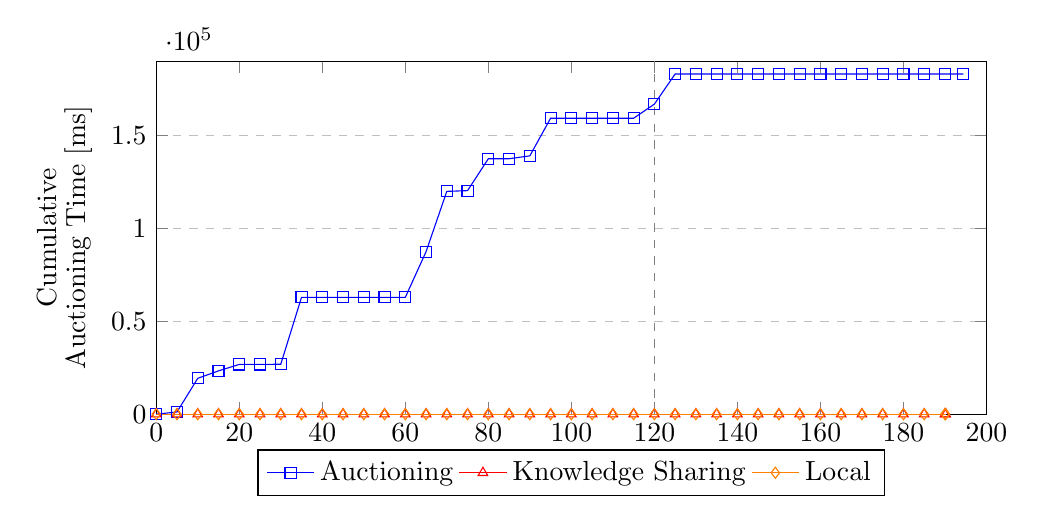
\begin{tikzpicture}
\begin{axis}[
    xlabel={Timestamp [s]},
    ylabel={\shortstack{Cumulative \\ Auctioning Time [ms]}},
    xmin=0, xmax=200000,
    ymin=0, ymax=190019,
    legend columns=-1,
    legend style={at={(0.5,-0.1)},anchor=north},
    ymajorgrids=true,
    grid style=dashed,
    width=\textwidth,
    height=0.5\textwidth,
    scaled x ticks=base 10:-3,
    xtick scale label code/.code={}
]

	\addplot[color=blue,mark=square] coordinates {
        (0,0)(5000,1183)(10000,19318)(15000,23323)(20000,26788)(25000,26788)(30000,26898)(35000,62914)(40000,62914)(45000,62914)(50000,62914)(55000,62914)(60000,62914)(65000,87496)(70000,119995)(75000,120385)(80000,137565)(85000,137565)(90000,139118)(95000,159369)(100000,159369)(105000,159369)(110000,159369)(115000,159369)(120000,166963)(125000,183205)(130000,183205)(135000,183205)(140000,183205)(145000,183205)(150000,183205)(155000,183205)(160000,183205)(165000,183205)(170000,183205)(175000,183205)(180000,183205)(185000,183205)(190000,183205)(194440,183205)
    };
    \addlegendentry{Auctioning}
	\addplot[color=red,mark=triangle] coordinates {
        (0,0)(5000,0)(10000,0)(15000,0)(20000,0)(25000,0)(30000,0)(35000,0)(40000,0)(45000,0)(50000,0)(55000,0)(60000,0)(65000,0)(70000,0)(75000,0)(80000,0)(85000,0)(90000,0)(95000,0)(100000,0)(105000,0)(110000,0)(115000,0)(120000,0)(125000,0)(130000,0)(135000,0)(140000,0)(145000,0)(150000,0)(155000,0)(160000,0)(165000,0)(170000,0)(175000,0)(180000,0)(185000,0)(190000,0)(190192,0)
    };
    \addlegendentry{Knowledge Sharing}
	\addplot[color=orange,mark=diamond] coordinates {
        (0,0)(5000,0)(10000,0)(15000,0)(20000,0)(25000,0)(30000,0)(35000,0)(40000,0)(45000,0)(50000,0)(55000,0)(60000,0)(65000,0)(70000,0)(75000,0)(80000,0)(85000,0)(90000,0)(95000,0)(100000,0)(105000,0)(110000,0)(115000,0)(120000,0)(125000,0)(130000,0)(135000,0)(140000,0)(145000,0)(150000,0)(155000,0)(160000,0)(165000,0)(170000,0)(175000,0)(180000,0)(185000,0)(190000,0)(190162,0)
    };
    \addlegendentry{Local}

	\addplot[color=gray, dashed,] coordinates {(120000,0) (120000,190019)};


\end{axis}
\end{tikzpicture}